\documentclass[aspectratio=169,11pt]{beamer}
\usepackage{amsmath,amssymb,tikz}
\usetikzlibrary{arrows.meta,positioning}
\definecolor{ink}{HTML}{142D4E}
\definecolor{accent}{HTML}{176B73}
\definecolor{modelbg}{HTML}{EDF6F5}
\definecolor{concretebg}{HTML}{F0F3F8}
\setbeamercolor{normal text}{fg=ink,bg=white}
\setbeamercolor{frametitle}{fg=ink}
\setbeamertemplate{navigation symbols}{}
\setbeamertemplate{footline}[frame number]
\setbeamersize{text margin left=7mm,text margin right=7mm}
\newcommand{\ok}{\operatorname{ok}}
\newcommand{\cadd}{\operatorname{add}}
\newcommand{\cmul}{\operatorname{mul}}
\newcommand{\bind}{\mathbin{\gg\!=}}
\tikzset{
  property/.style={draw=accent!60,rounded corners=5pt,line width=0.8pt,
    text width=12.3cm,align=center,inner sep=11pt},
  refinement/.style={-{Latex[length=3mm]},line width=1.2pt,accent}
}
\begin{document}
\begin{frame}{Why start with smaller examples?}
\centering
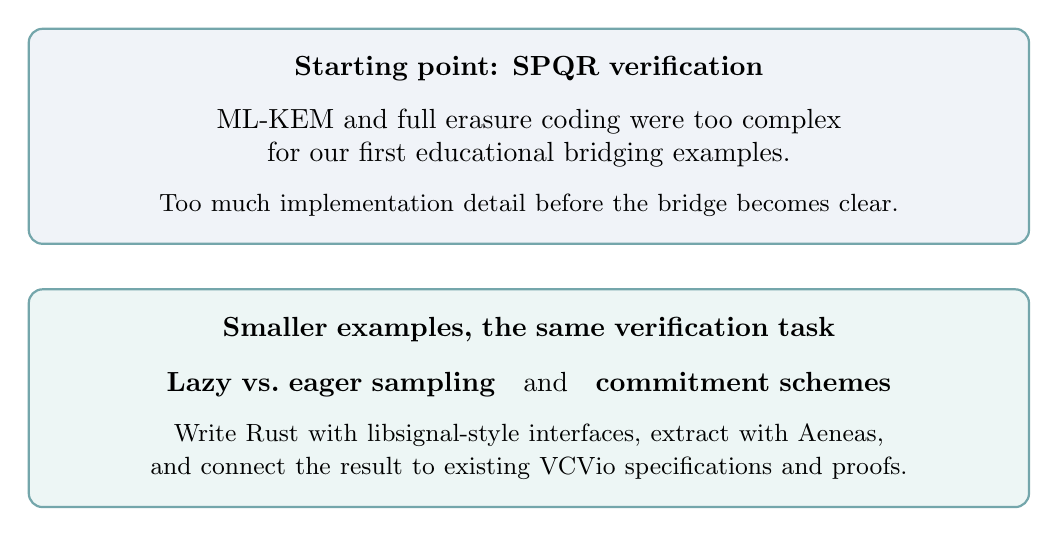
\begin{tikzpicture}
\node[property,fill=concretebg,text width=12.0cm,inner sep=10pt] (large) {
  \textbf{Starting point: SPQR verification}\\[7pt]
  ML-KEM and full erasure coding were too complex\\
  for our first educational bridging examples.\\[6pt]
  {\small Too much implementation detail before the bridge becomes clear.}
};
\node[property,fill=modelbg,text width=12.0cm,inner sep=10pt,
  below=0.55cm of large] (small) {
  \textbf{Smaller examples, the same verification task}\\[8pt]
  \textbf{Lazy vs.\ eager sampling}\quad and\quad \textbf{commitment schemes}\\[7pt]
  {\small Write Rust with libsignal-style interfaces, extract with Aeneas,\\
  and connect the result to existing VCVio specifications and proofs.}
};
\end{tikzpicture}

\vspace{0.3cm}
{\small\textbf{Goal:} teach the bridge from implementation to specification.}

\end{frame}

\begin{frame}{Bridging implementation and specification}
\centering
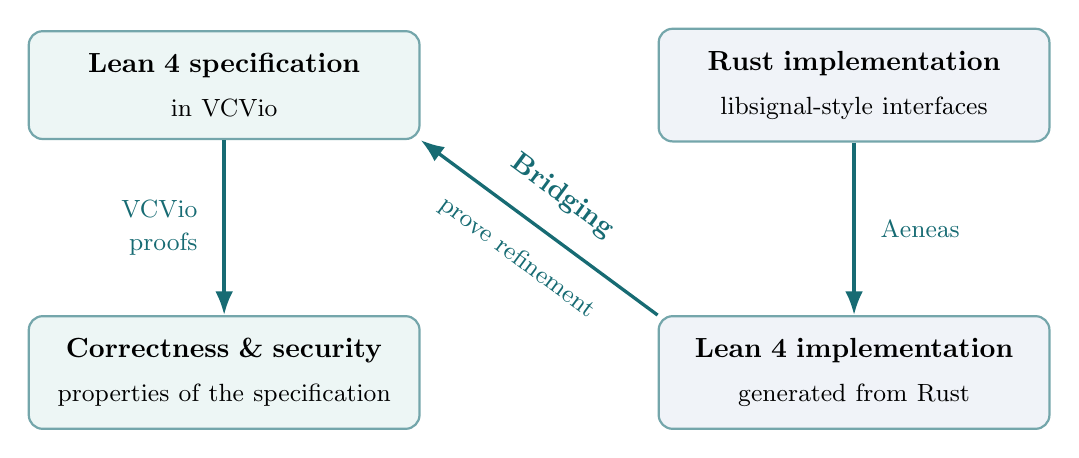
\begin{tikzpicture}[
  box/.style={draw=accent!60,rounded corners=5pt,line width=0.8pt,
    text width=4.4cm,minimum height=1.35cm,align=center,inner sep=8pt},
  edge/.style={-{Latex[length=3mm]},line width=1.2pt,accent}
]
\node[box,fill=modelbg] (spec) at (0,0) {
  \textbf{Lean 4 specification}\\[4pt]
  {\small in VCVio}
};
\node[box,fill=concretebg] (rust) at (8,0) {
  \textbf{Rust implementation}\\[4pt]
  {\small libsignal-style interfaces}
};
\node[box,fill=concretebg] (lean) at (8,-3.65) {
  \textbf{Lean 4 implementation}\\[4pt]
  {\small generated from Rust}
};
\node[box,fill=modelbg] (properties) at (0,-3.65) {
  \textbf{Correctness \& security}\\[4pt]
  {\small properties of the specification}
};
\draw[edge] (rust.south) -- (lean.north)
  node[midway,right=2mm] {\small Aeneas};
\draw[edge] (lean.north west) -- (spec.south east)
  node[midway,above=2mm,sloped] {\textbf{Bridging}}
  node[midway,below=2mm,sloped] {\small prove refinement};
\draw[edge] (spec.south) -- (properties.north)
  node[midway,left=2mm,align=right] {\small VCVio\\\small proofs};
\end{tikzpicture}

\vspace{0.3cm}
{\small The bridge lets specification-level guarantees apply to the implementation.}

\vspace{0.15cm}
{\scriptsize Representation maps and RNG/oracle assumptions are explicit.}
\end{frame}

\end{document}
